\subsection{Fragen und Antworten zum Text von \textcite{fetterman_empowerment_2007}}
\subsubsection{Unter ``Conceptual Amibuity, Metodological Specificity, and Outcomes'': Welche Probleme werden in der Studie von Miller und Campbell (2006) identifiziert?}
\begin{itemize}
        \item Mehrheit der Studien war alt
        \item wichtige Beispiele fehlten
        \item es wurden nur Artikel und B"ucher einbezogen, keine Evaluation Reports
        \item 10 Kriterien von Fetterman und Wandersman waren nicht erf"ullt
        \item nur weil Empowerment drauf steht, ist noch lange nicht Empowerment drin
\end{itemize}

\subsubsection{``Empowerig others'' bedeutetet f"ur die Empowerment Evaluation\ldots}
\ldots dass man Anderen hilft, \emph{sich selbst zu empowern}. Es ist n"amlich nicht m"oglich, jemand anderen zu empowern. Anders gesagt: die bereits vorhandene Energie soll freigesetzt werden.

\subsubsection{Empowerment Evaluation bindet nicht nur Programmmitarbeitende ein. Welche anderen Gruppen sind noch beteiligt?}
\begin{itemize}
        \item Stakeholder
        \item Sponsoren
        \item Forscher
\end{itemize}

\subsubsection{Kann Empowerment Evaluation ausschlie"slich transformativ sein? Warum?}
Empowerment Evaluation kann entweder transformativ oder praktischer Natur sein. Es kommt auf den Zweck der Evaluation an. Wenn es um Entscheidungshilfe geht, dann handelt es sich um eine praktische Natur. Wenn es um psychologische oder politische Ver"anderungen geht, dann handelt es sich um transformative Evaluation.

\subsubsection{Warum ist Empowerment Evaluation nach Fetterman und Wandersman Evaluation und nicht Movement?}
Es gibt wohl drei Kriterien von Chelimsky (1997), die zumindest teilweise erf"ullt sein m"ussen, damit man von einer Evaluation sprechen kann. Diese drei Kriterien sind \emph{Entwicklung}, \emph{Accountability} und \emph{Wissen}. Nach \textcite{fetterman_empowerment_2007} gibt es ausreichend Befunde daf"ur, dass EE mindestens zwei der Kriterien erf"ullt.

\subsubsection{Mit welchen drei Argumenten disutieren Fetterman und Wandersman die Brauchbarkeit des Begriffs \emph{Ideology} im Zusammenhang mit Empowerment Evaluation?}
EE wird als Ideologie dem experimentellen Ansatz gegen"ubergestellt. Die drei Argumente dagegen sind:
\begin{itemize}
        \item EE und experimentelle Ans"atze schlie"sen sich nicht gegenseitig aus
        \item Experimentelle Ans"atze sind auch in EE's durchgef"uhrt worden
        \item Experimentelle Ans"atze sind au"serdem benutzt worden, um die Efficacy von EE zu untersuchen
\end{itemize}

\subsubsection{Was sind Gemeinsamkeiten, was Unterschiede im Vergleich von kollaborativen Evaluationsformen und Empowerment Evaluation?}
Hier geht es vor allem um \emph{Kollaborative Evaluation}, \emph{Partizipative Evaluation} und \emph{Empowerment Evaluation}. Gemeinsam ist allen Formen, dass sie wert auf \emph{Partizipation} und \emph{Kontrolle} legen. Die EE ist dabei auf beiden Dimensionen am weitesten rechts angesiedelt, gefolgt von der Partizipativen Evaluation. (Siehe Fig. \ref{fig:fetterman1})

EE hat allerdings zus"atzlich einen Fokus auf \emph{Selbstbestimmtheit} und \emph{Selbstevaluation}.

\begin{figure}[h!]
        \begin{center}
                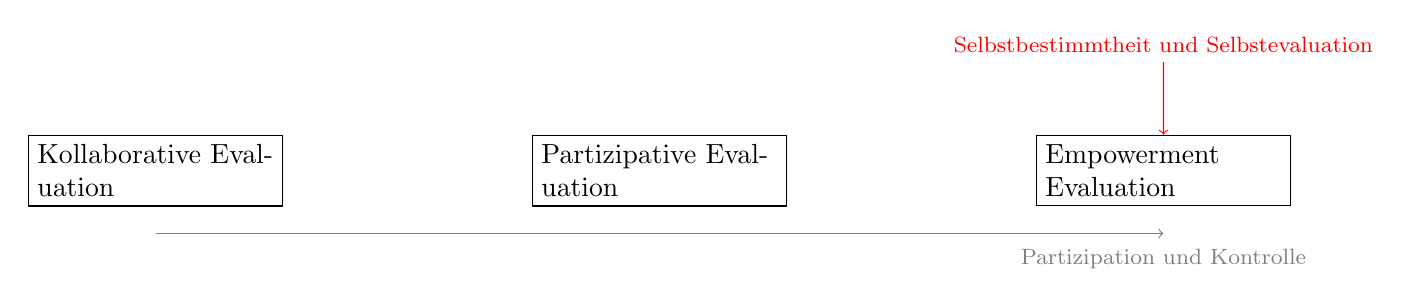
\begin{tikzpicture}[eval/.style={shape=rectangle,draw,text width=3cm},
                        dim/.style={font=\footnotesize,color=gray},
                        selbst/.style={shape=rectangle,rounded corners,font=\footnotesize,color=red},
                        scale=.8]
                        \draw[->,gray] (-8,0) -- (+8,0);
                        \node[dim] at (+8, -0.4) {Partizipation und Kontrolle};
                        \node[eval] at (-8, 1) {Kollaborative Evaluation};
                        \node[eval] at (0, 1) {Partizipative Evaluation};
                        \node[eval] at (+8,1) (ee) {Empowerment Evaluation};
                        \node[selbst] at(+8,3) (selbst) {Selbstbestimmtheit und Selbstevaluation};
                        \draw[->,red] (selbst) -- (ee);
                \end{tikzpicture}
        \end{center}
        \caption{Die drei Formen der Evaluation und ihre Position auf den Dimensionen \emph{Partizipation} und \emph{Kontrolle} (beide dargestellt durch dieselbe Achse). Empowerment Evaluation zeichnet sich durch den besonderen Folus auf Selbstbestimmtheit und Selbstevaluation aus.}
        \label{fig:fetterman1}
\end{figure}

\subsubsection{Mit welchen Argumenten begegnen Fettersman und Wandersman der heutigen Kritik, EE sei nicht klar genug im Hinblick auf ihr Konzept und ihre Prinzipien?}
Im Hinblick auf das Konzept haben Fetterman und Wandersman in ihrem Buch von 2005 einige Begriffe spzeifiziert. Darunter fallen \emph{Selbstbestimmtheit}, \emph{Empowerment} und \emph{Community}. Sie haben au"serdem $10$ Prinzipien formuliert:
\begin{enumerate}
        \item Verbesserung
        \item Community ownership
        \item Inklusion
        \item demokratische Partizipation
        \item soziale Gerechtigkeit
        \item Wissen "uber die Community
        \item evidenzbasierte Strategien
        \item Capacity building
        \item organisationales Lernen
        \item Accountability
\end{enumerate}

\subsubsection{Welches sind die 3 Schritte des \emph{3-step approach}?}
\begin{enumerate}
        \item Was ist das Ziel?
        \item Bestandsaufnahme
        \item Plan f"ur die Zukunft
\end{enumerate}

\subsubsection{Eine Kritik lautet: EE k"ummert sich zu wenig um Outcomes. Welche $4$ Outcomes f"uhren Fetterman und Wandersman an?}
\begin{itemize}
        \item Capacity Outcomes
        \item Standardized Test Scores
        \item Programm Outcomes
        \item Accreditation Outcomes (Ausma"s an Beteiligung und Engagement)
\end{itemize}

\subsubsection{Was haben die Programmdurchf"uhrenden des Programms MISGRO unternommen, um einer Schw"ache des Programms zu begegnen, die im Rahmen der taking-stock Phase identifiziert wurde?}
Sie haben \emph{Evaluation Monitoring System} entwickelt, mit dem die Anzahl derer, die mit dem Rauchen aufgeh"ort haben, erfasst wurde. Dieses Ma"s wurde erweitert durch die Anzahl an geretteten Leben und durch den Betrag, der dadurch gespart wurde. 

